%\documentclass[11pt,fleqn,twoside]{article}
\documentclass{llncs}

\usepackage[english]{babel}
\usepackage{alltt}
\usepackage{graphicx}
\usepackage{url}
\usepackage{subfigure}
\usepackage{listings}
\usepackage{color}
\usepackage{lscape}
\usepackage{xspace}
\usepackage{latexsym}
\usepackage{rotating} 
\usepackage{enumitem}

\usepackage{verbatim}
\usepackage{url}
\usepackage{multirow} 


\usepackage{colortbl}
\usepackage[table]{xcolor}

\makeatletter
\renewcommand{\thetable}{\thesection.\@arabic\c@table}
\@addtoreset{table}{section}
\makeatother


\definecolor{MyDarkBlue}{rgb}{0,0.08,0.45} 
\newcommand{\dv}[1] {\textcolor{blue}{[DV]\textit{#1}}}
\newcommand{\bo}[1] {\textcolor{MyDarkBlue}{[BO]\textit{#1}}}

\begin{document}

\title{Notes on Physical \& Logical Data Layouts}
	\author{
	Michael Hausenblas\inst{1} 
	}
	\institute{MapR Technologies EMEA, Ireland\\
	\email{mhausenblas@maprtech.com}
	}
\maketitle

\begin{abstract}
In this short note I review and discuss principled options for physical and
logical data layouts as well as implications on data processing at large scales.
I should say in advance that these notes offer no new insights, that is, 
everything stated here has already been published elsewhere. In fact, it has
been published in so many different places, such as blog posts, in the 
literature, etc. that the main contribution is to bring it all together in one
place.
\end{abstract}

\section{Motivation}
\label{sec:mot}
Conceptually, there are three levels present in data management systems
(Fig.~\ref{fig:data-layers}):
\begin{figure}[h!]
\centering
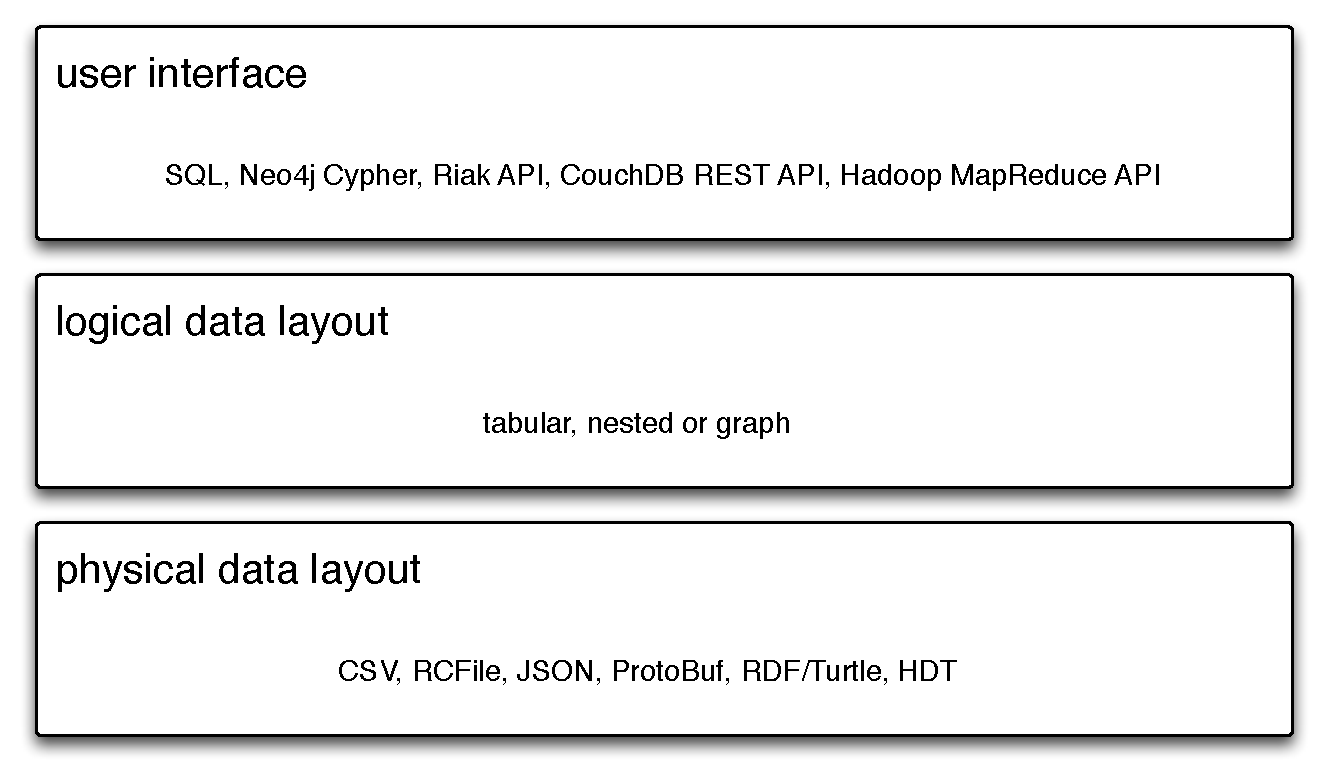
\includegraphics[width=0.7\textwidth]{data-layers}
\caption{The three levels of data representation and interaction in data 
management systems, including examples for each of the levels.}
\label{fig:data-layers}
\end{figure}
\begin{itemize}
\item The \emph{User Interface} level. Any database or datastore needs 
to provide a way to interact with the data under management. This can be 
something elaborate, standardised and mature as the Structured Query Language 
(SQL) found in relational database management systems (RDBMS), such as 
Oracle DB, PostgreSQL, or MySQL. This can be a RESTful interface, found in many 
NoSQL datastores, like, for example, CouchDB's API\footnote{See online 
documentation at \url{http://wiki.apache.org/couchdb/HTTP_Document_API}}. Of
course, this can also be a programming-language-level API such as the case with
Hadoop\footnote{\url{http://hadoop.apache.org/docs/current/api/org/apache/hadoop
/mapreduce/package-summary.html}}.
\item The \emph{Logical Data Layout} level.
\item The \emph{Physical Data Layout} level.
\end{itemize}




\section{Manifestations of Data Layouts}
\label{sec:mani}




\begin{figure}[h!]
\centering
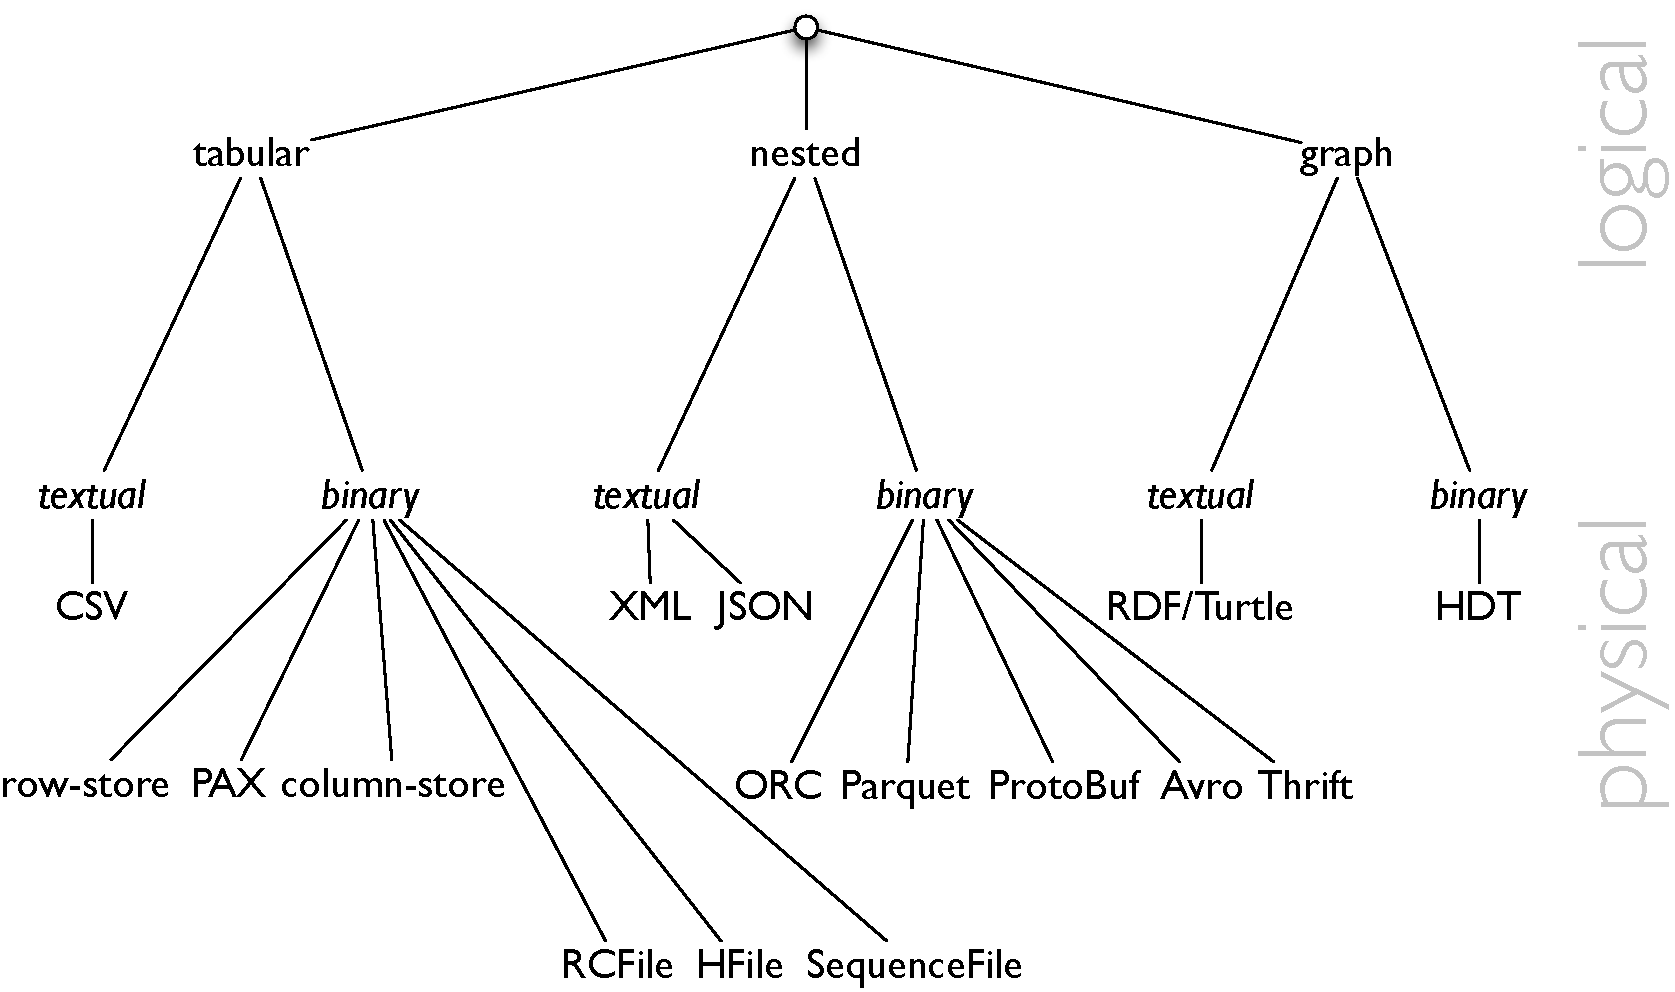
\includegraphics[width=0.9\textwidth]{taxonomy-dl}
\caption{A non-exhaustive, lightweight taxonomy for logical and physical data 
layouts and serialisation formats commonly used in the data processing 
community.}
\label{fig:taxonomy-dl}
\end{figure}

\section{Logical Layouts}
\label{sec:loglay}

\section{Physical Layouts}
\label{sec:phylay}

\section{Layering Physical and Logical Layouts}
\label{sec:laylay}


\section{Impact on Data Processing at Scale}
\label{sec:ldp}


\section{Conclusions and Challenges}
\label{sec:concl}

\section{Acknowledgements}
\label{sec:ack}
I'd like to thank Eric Brewer, whose RICON2012 keynote motivated me to write up
this short note. His keynote is available via \url{https://vimeo.com/52446728} 
and more than certainly worth it watching it.

\bibliographystyle{alpha}
\bibliography{data-proc}


\end{document}

